
%------------------------------------------------

\section{Sum of normally distributed random variables}
\label{exer:sum_of_Gaussian}

\subsection{Normally distributed and uncorrelated does not imply independent}

Two normally distributed, uncorrelated but dependent variables.

Suppose $X$ has a normal distribution with expected value 0 and variance 1. Let $W$ have the Rademacher distribution, so that 

\begin{equation}\label{eq:Rademacher_distr}
	w(x) = \left\{
	\begin{array}{ccl}
		\frac{1}{2} & & {\textrm{if } W = 1}\\
		\frac{1}{2} & & {\textrm{if } W = - 1}\\
		0 & & {\textrm{otherwise}}
	\end{array} \right.
\end{equation}

and assume $W$ is independent of $X$. Let $Y=WX$. Then
\begin{itemize}
	\item $X$ and $Y$ are uncorrelated;
	\item both have the same normal distribution;
	\item and $X$ and $Y$ are not independent.
\end{itemize}

The joint probability distribution is shown in Figure~\ref{fig:joint_pdf_sum_of_Gaussian}.

\begin{figure}
	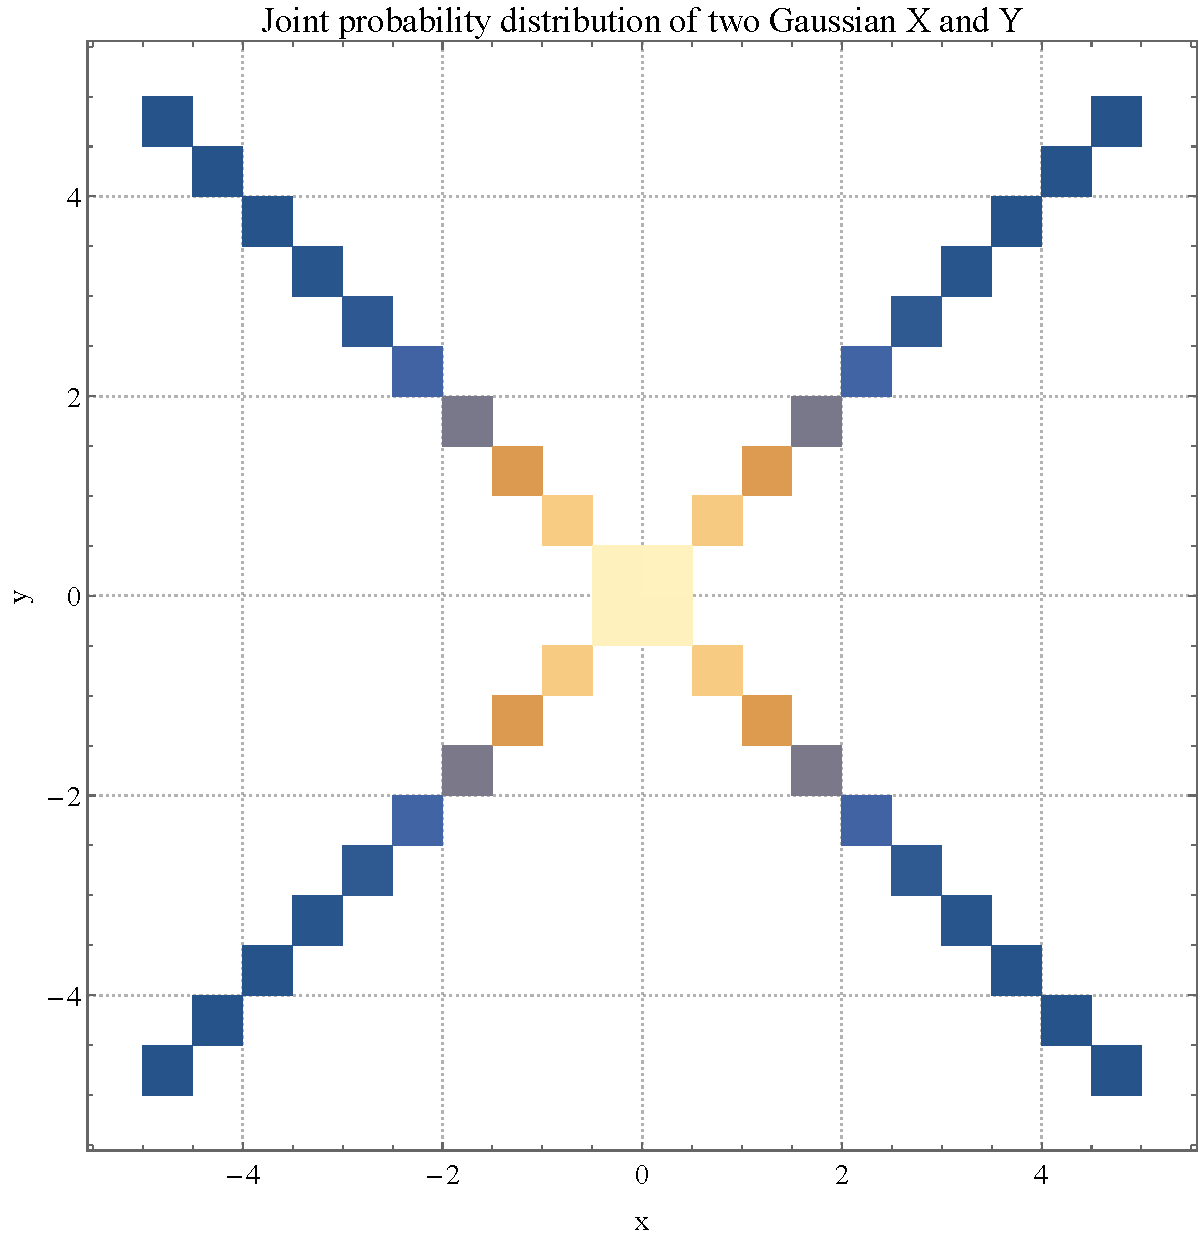
\includegraphics{exercise/joint_pdf_of_two_Gaussian.pdf}
	\caption[Joint probability distribution of two “normal” variables $X$ and $Y$.][6pt]{Joint probability distribution of two “normal” variables $X$ and $Y$.}
	\label{fig:joint_pdf_sum_of_Gaussian}
\end{figure}

To see that $X$ and $Y$ are uncorrelated, one may consider the covariance $\mathrm{cov} (X,Y)$: by definition, it is

$$
\mathrm{cov}(X, Y) = \mathrm{E}(XY) - \mathrm{E}(X) \mathrm{E}(Y)
$$

Then by definition of the random variables $X$, $Y$, and $W$, and the independence of $W$ from $X$, one has

$$
\mathrm{cov}(X, Y)= \mathrm{E}(XY) - 0 = \mathrm{E}(X^{2} W) = \mathrm{E}(X^{2}) \mathrm{E}(W) = \mathrm{E}(X^{2}) \cdot 0 = 0
$$

To see that $Y$ has the same normal distribution as $X$, consider

$$
\begin{array}{rl}
	P(Y \leq x) &= \mathrm{E}(P(Y \leq x \mid W))\\
	&= P(X \leq x) P(W = 1) + P(- X \leq x) P(W = -1)\\
	&= \Phi(x) \cdot \frac{1}{2} + \Phi(x) \cdot \frac{1}{2}
\end{array}
$$

\marginnote{Since $X$ and $- X$ both have the same normal distribution.}

where $\Phi(x)$ is the cumulative distribution function of the standard normal distribution.

To see that $X$ and $Y$ are not independent, observe that

$$
P(Y > 1 \mid - \frac{1}{2} < X < \frac{1}{2}) = P( X > 1 | - \frac{1}{2} < X < \frac{1}{2}) = 0
$$

Finally, the distribution of the simple linear combination $X + Y$ concentrates positive probability at 0 (Figure~\ref{fig:sum_of_Gaussian}): 

$$
P(X + Y = 0) = \frac{1}{2}
$$

Therefore, the random variable $X + Y$ is not normally distributed, and so also $X$ and $Y$ are not jointly normally distributed. 

\begin{figure}
	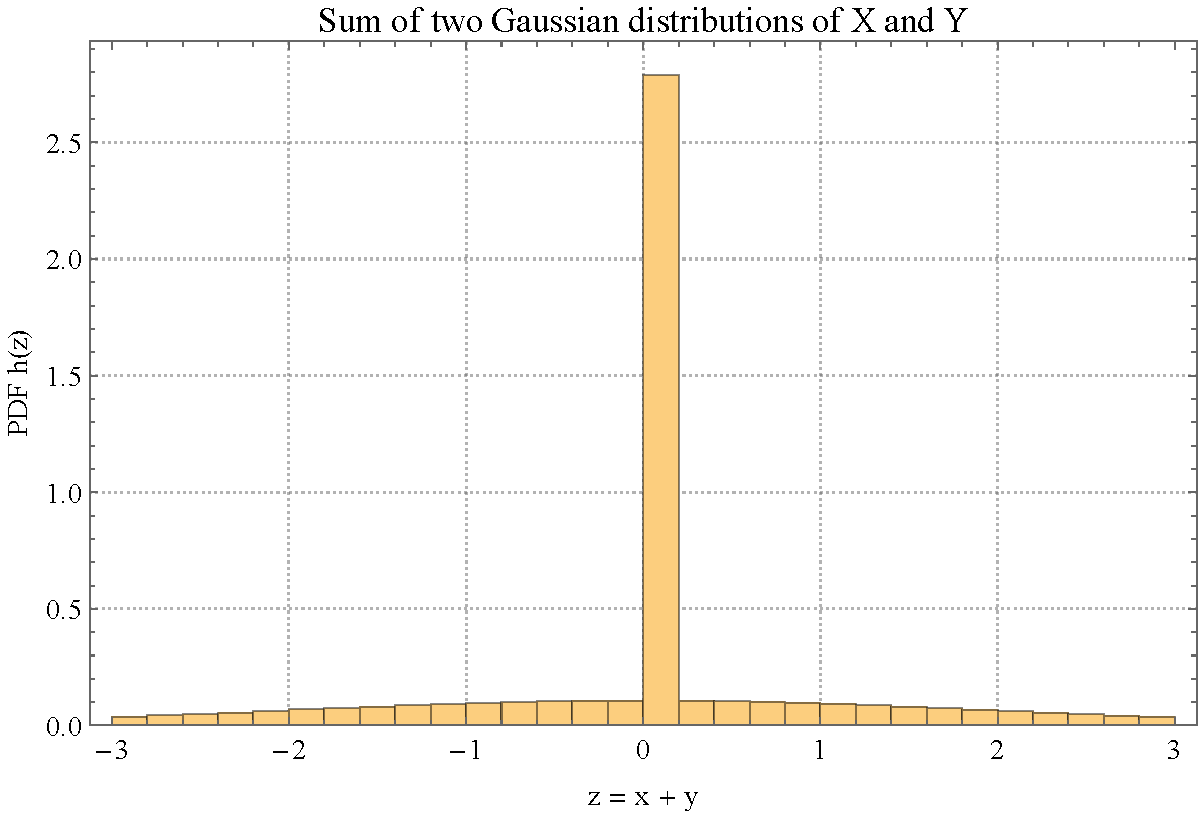
\includegraphics{exercise/sum_of_Gaussian.pdf}
	\caption[Probability distribution of the sum of two “normal” variables.][6pt]{Probability distribution of the sum of two “normal” variables $X$ and $Y$.}
	\label{fig:sum_of_Gaussian}
\end{figure}

($\hookleftarrow$ \ref{subsec:prop_of_gaussian_distr})
